\chapter{Results}

\section{Isothermal Jet}
Our first case involves the isothermal jet where both jet and ambient fluid are at $330 K$. Quantities of interest for this case are compared against incompressible round jet statistics as outlined in Pope \cite{Pope} and isothermal compressible jet turbulence features \cite{}. This case serves as a baseline for comparison with the other two cases involving non-isothermal jets. 
\subsection{Flow Field Features}
All images herein depict a slice of the 3D flow field at $z=0$. Each figure contains an instantaneous snapshot and a time-averaged snapshot of the entire slice domain, plus an additional zoomed-in image of the time-averaged quantity of interest near the inlet. All instantaneous images are taken from the final data point of the simulation.

Figure \ref{330_v_features} shows the axial velocity component of the flow field. The general spreading rate and decay of the velocity field can be seen from the instantaneous snapshot in \ref{330_v_1}. The flow is mostly steady up until $\nicefrac{y}{d}=2$ before perturbations begin. The stream mostly stays together through these initial perturbations up until $\nicefrac{y}{d}=5$ where spreading then begins. The averaged axial velocity fields in \ref{330_v_3} and \ref{330_v_4} shed more light on the approximate development regions of the jet. The potential core extends up to $\nicefrac{y}{d}=5$, followed by the transition region where $5 \leq \nicefrac{y}{d} \leq 10$, thereafter the jet appears fully developed. Centerline analysis of the turbulent kinetic energy later on will provide more information for these boundaries.  

\begin{figure}[htbp!]
\begin{subfigure}{0.25\textwidth}
	\centering
	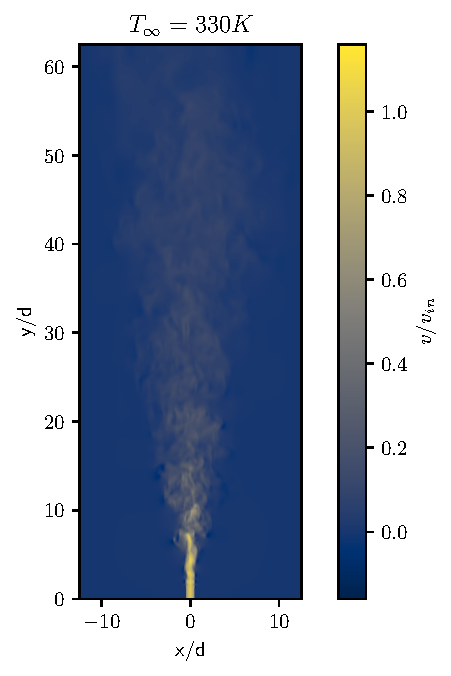
\includegraphics[scale=.65]{figures/Plots/vertical/330/v_scaled_vert_330.pdf}
	\caption{Scaled instantaneous axial velocity} \label{330_v_1}
\end{subfigure}
\hfill
% \begin{subfigure}{0.3\textwidth}
% 	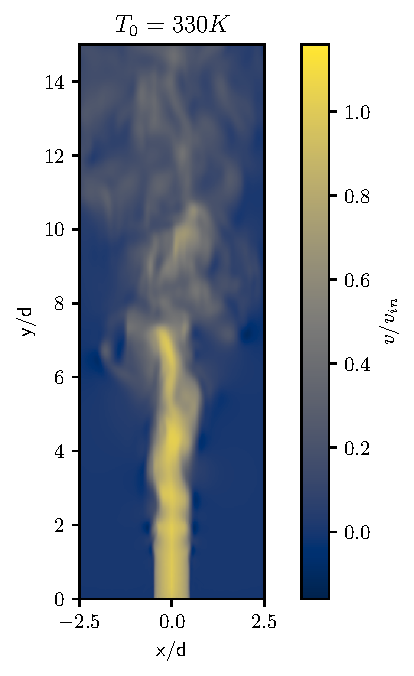
\includegraphics[scale=.75]{figures/Plots/vertical/330/v_scaled_vert_330_zoom.pdf}
% 	\caption{Close up of scaled instantaneous axial velocity near inlet} \label{330_v_2}
% \end{subfigure}
\begin{subfigure}{0.25\textwidth}
	\centering
	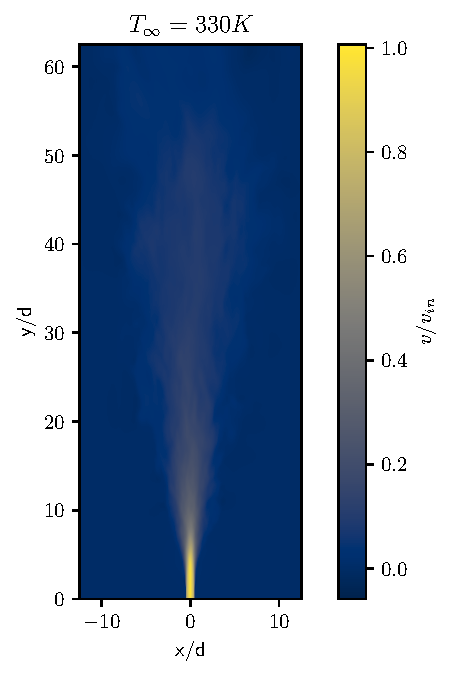
\includegraphics[scale=.65]{figures/Plots/vertical/330/v_scaled_vert_avg_330.pdf}
	\caption{Scaled average axial velocity} \label{330_v_3}
\end{subfigure}
\hfill
\begin{subfigure}{0.25\textwidth}
	\centering
	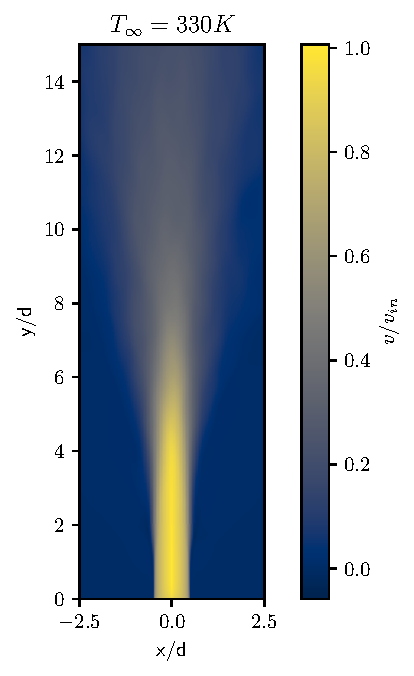
\includegraphics[scale=.65]{figures/Plots/vertical/330/v_scaled_vert_avg_330_zoom.pdf}
	\caption{Close up of scaled average axial velocity near inlet} \label{330_v_4}
\end{subfigure}
\caption{Axial velocity features of the isothermal jet}
\label{330_v_features}
\end{figure}

Figure \ref{330_pressure_features} shows minor pressure fluctuations in the flow, scaled against the maximum pressure achieved above the ambient pressure. \ref{330_pressure_1} shows minor pressure oscillations mirrored on each side of the jet edge in the same zone as the initial velocity fluctuations see in \ref{330_v_1}. Thereafter, the oscillations become off-kilter, correlating to the beginning of the jet disintegration as seen in the velocity field. Pressure fluctuations are concentrated near the inlet and die down past the transition zone. This can be seen more clearly in \ref{330_pressure_3}. On average, pressure fluctuations yield a minor increase within the potential core and decrease on the jet perimeter, as can be seen in \ref{330_pressure_4}. Fluctuations also lead to a minor pressure drop on average in the transition region.  

\begin{figure}[htbp!]
\begin{subfigure}{0.25\textwidth}
	\centering
	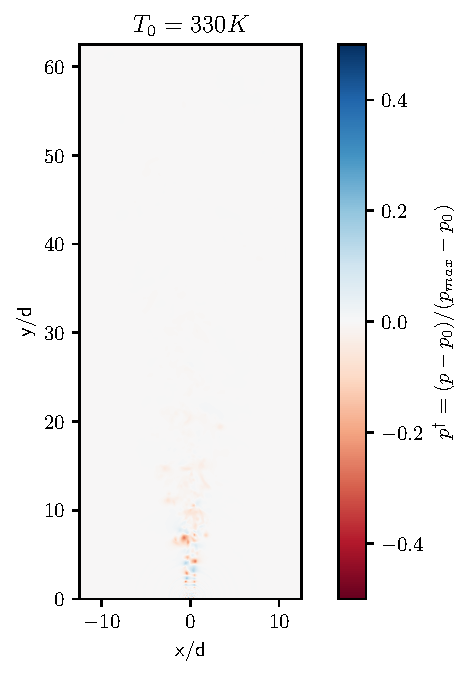
\includegraphics[scale=.65]{figures/Plots/vertical/330/pressure_scaled_vert_330.pdf}
	\caption{Scaled instantaneous pressure fluctuations} \label{330_pressure_1}
\end{subfigure}
\hfill
% \begin{subfigure}{0.25\textwidth}
% 	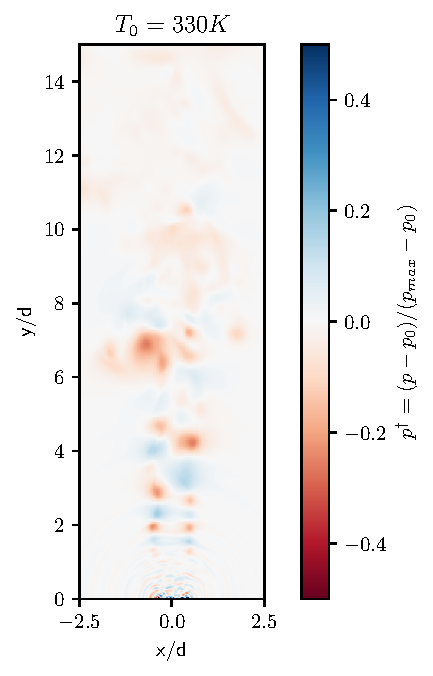
\includegraphics[scale=.65]{figures/Plots/vertical/330/pressure_scaled_vert_330_zoom.pdf}
% 	\caption{Close up of scaled instantaneous pressure fluctuations near inlet} \label{330_pressure_2}
% \end{subfigure}
\begin{subfigure}{0.25\textwidth}
	\centering
	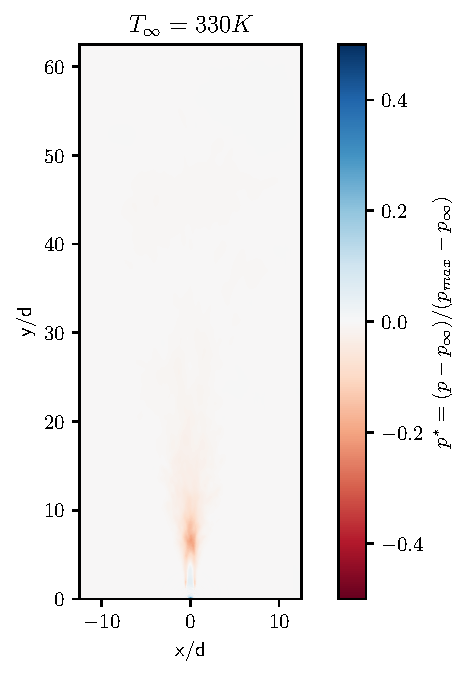
\includegraphics[scale=.65]{figures/Plots/vertical/330/pressure_scaled_vert_avg_330.pdf}
	\caption{Scaled average pressure fluctuations} \label{330_pressure_3}
\end{subfigure}
\hfill
\begin{subfigure}{0.25\textwidth}
	\centering
	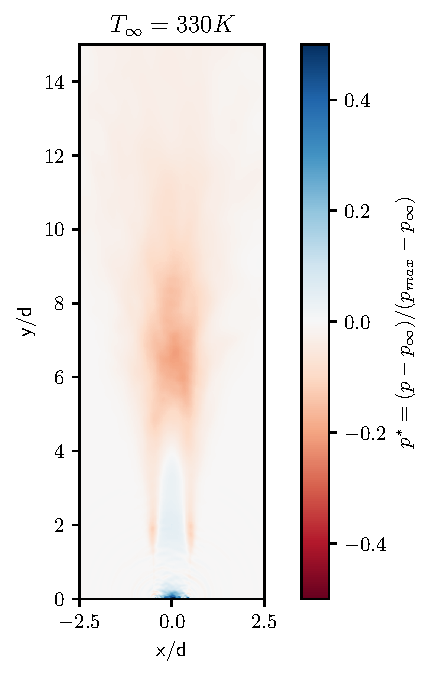
\includegraphics[scale=.65]{figures/Plots/vertical/330/pressure_scaled_vert_avg_330_zoom.pdf}
	\caption{Close up of scaled average pressure fluctuations near inlet} \label{330_pressure_4}
\end{subfigure}
\caption{Pressure features of the isothermal jet}
\label{330_pressure_features}
\end{figure}

Figure \ref{330_magvort_features} shows magnitude of the vorticity scaled between the maximal and minimal values. \ref{330_magvort_1} shows the strongest vorticity occurring at the jet interface with the ambient fluid near the inlet. Past this initial stage, vortex shedding occurs and vorticity dissipates as the jet spreads. The averages in \ref{330_magvort_3} and \ref{330_magvort_4} both show again that the most intense vorticity occurs at the inlet along the outer edge of the jet. This high intensity remains constant until about $\nicefrac{y}{d}=1$ before more mixing with the ambient fluid occurs as the jet spreads and the vorticity lessens in intensity. Vortices are still restricted to the jet edge until around $\nicefrac{y}{d} = 5$ where the transition to fully developed turbulence enables vortical motions to extend across the fully spread of the jet. 

\begin{figure}[htbp!]
\begin{subfigure}{0.25\textwidth}
	\centering
	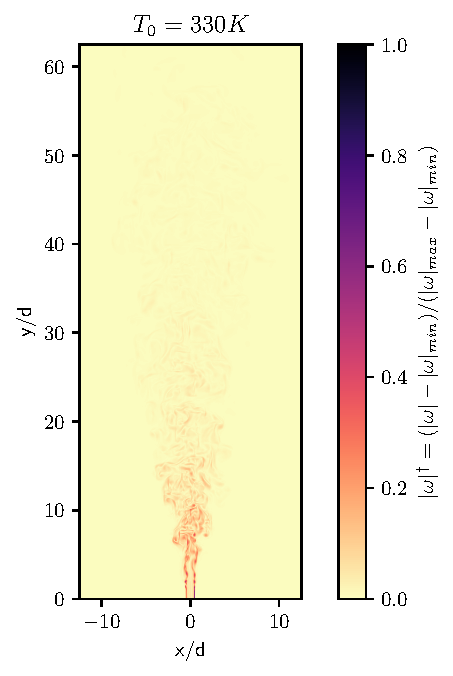
\includegraphics[scale=.65]{figures/Plots/vertical/330/magvort_scaled_vert_330.pdf}
	\caption{Scaled instantaneous vorticity magnitude} \label{330_magvort_1}
\end{subfigure}
\hfill
% \begin{subfigure}{0.25\textwidth}
%	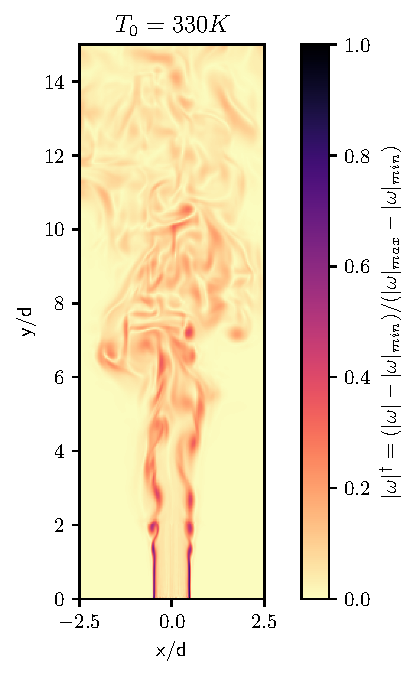
\includegraphics[scale=.65]{figures/Plots/vertical/330/magvort_scaled_vert_330_zoom.pdf}
%	\caption{Close up of scaled instantaneous vorticity magnitude near inlet} \label{330_magvort_2}
%\end{subfigure}
\begin{subfigure}{0.25\textwidth}
	\centering
	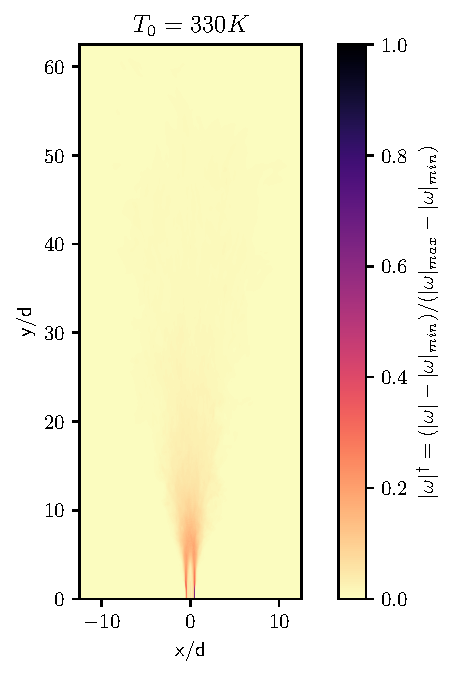
\includegraphics[scale=.65]{figures/Plots/vertical/330/magvort_scaled_vert_avg_330.pdf}
	\caption{Scaled average vorticity magnitude} \label{330_magvort_3}
\end{subfigure}
\hfill
\begin{subfigure}{0.25\textwidth}
	\centering
	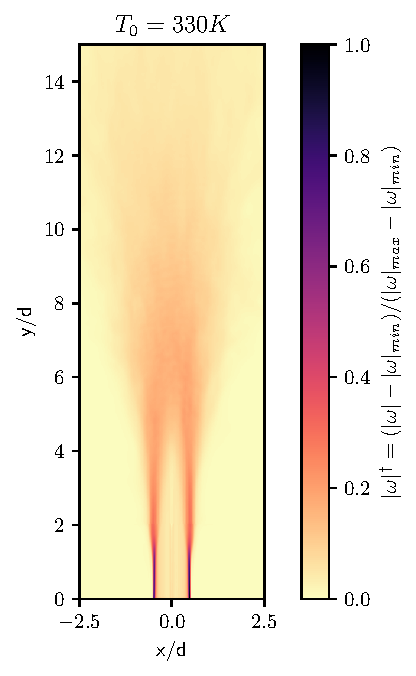
\includegraphics[scale=.65]{figures/Plots/vertical/330/magvort_scaled_vert_avg_330_zoom.pdf}
	\caption{Close up of scaled average vorticity magnitude near inlet} \label{330_magvort_4}
\end{subfigure}
\caption{Vorticity magnitude features of the isothermal jet}
\label{330_magvort_features}
\end{figure}

\subsection{Mean Flow Properties}
Figure \ref{330_centerline_decay} depicts the time and radially averaged scaled axial velocity component plotted against radial distance from the centerline at multiple normal slices downstream from the inlet. The velocity is scaled by the average axially velocity value at the inflow while the radial direction is scaled by the jet diameter. These plots demonstrate the axially velocity decay as the flow progresses further downstream. As velocity value along the centerline decreases, the overall velocity profile also widens and flattens out. Typically, for the round turbulent jet, this expansion would occur in such a way that upon specially selected scaling, these profiles would collapse into one profile after a certain point. This potential is explored further in the next figure. Here though this decay is a common feature of how the axial velocity of the jet develops as it leaves the inlet. 

\begin{figure}[htbp!]
\begin{center}
	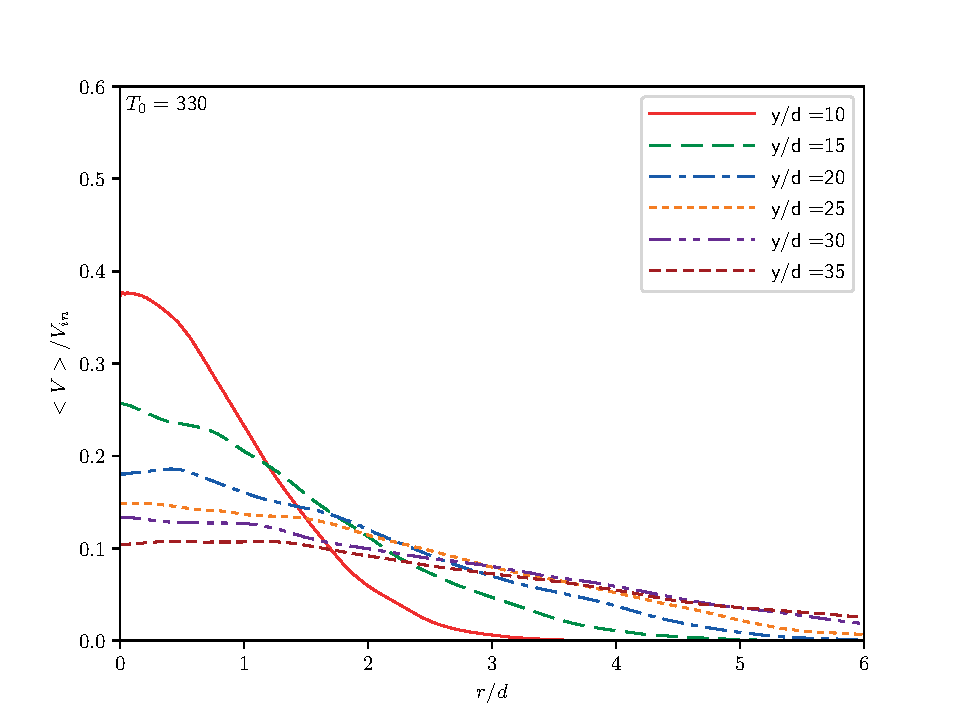
\includegraphics[scale=.7]{figures/Plots/radial/slices_5/same_ambient/ur_u_in_vs_r_d.pdf}
	\caption{Average (both in time and radially) axial velocity scaled by inlet value plotted along radial distance from centerline. Profile decay follows similar trajectory to what is expected in incompressible round jet theory \cite{Pope}.} \label{330_centerline_decay}
\end{center}
\end{figure}

Figure \ref{330_r_v_features} depicts time and radially averaged scaled axial velocity components plotted against the radial distance from the centerline. Each curve is made at a slice normal to the axial flow direction at different points downstream. Figure \ref{330_r_vs_v_1} depicts velocity curves every $3d$ downstream from the inlet near where the transition region begins while Figure \ref{330_r_vs_v_2} contains plots taken every $5d$. The axial velocity is scaled by the centerline value $v_c$ while the radial distance is scaled by the half width half mean (HWHM), where the velocity component is equal to half the value on the centerline $v(r_{1/2}) = \nicefrac{v_c}{2}$.

Figure \ref{330_r_vs_v_1} shows the near-field axial velocity profiles. They already exhibit self-similarity collapse into one profile which is most likely the result of the inflow condition \cite{}. In the far-field slices of \ref{330_r_vs_v_2}, self-similarity is fairly well maintained with minor fluctuations in the center and edge of the jet. These fluctuations are most likely the result of low resolution in the time averaging of available data. 

\begin{figure}[htbp!]
\begin{center}
\begin{subfigure}{0.45\textwidth}
	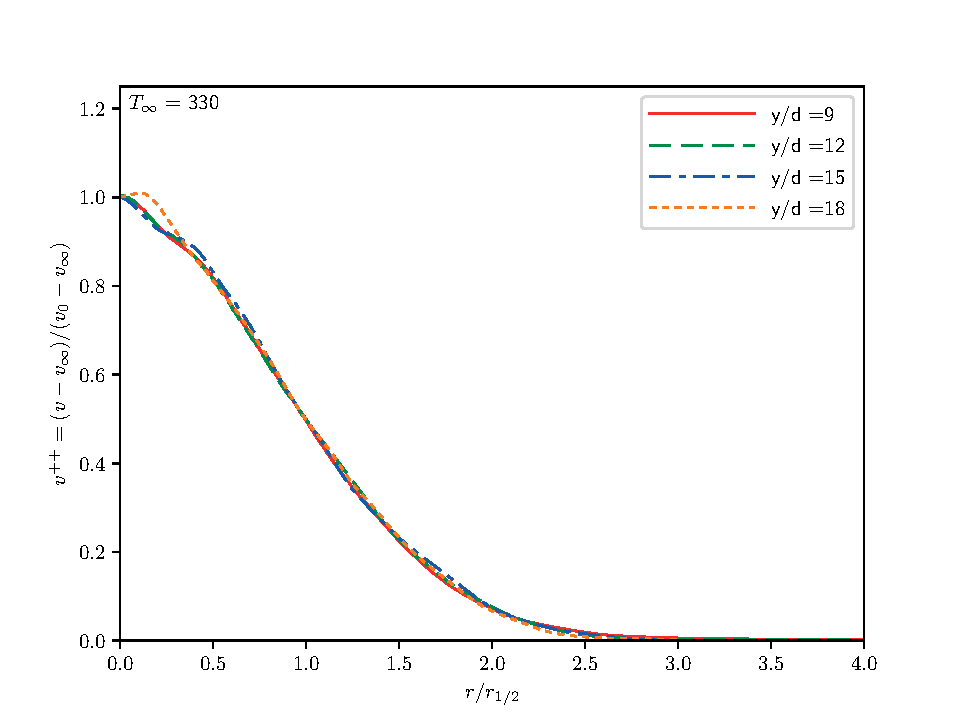
\includegraphics[scale=.45]{figures/Plots/radial/slices_3/same_ambient/r_vs_v.pdf}
	\caption{Near-Field} \label{330_r_vs_v_1}
\end{subfigure}
\begin{subfigure}{0.45\textwidth}
	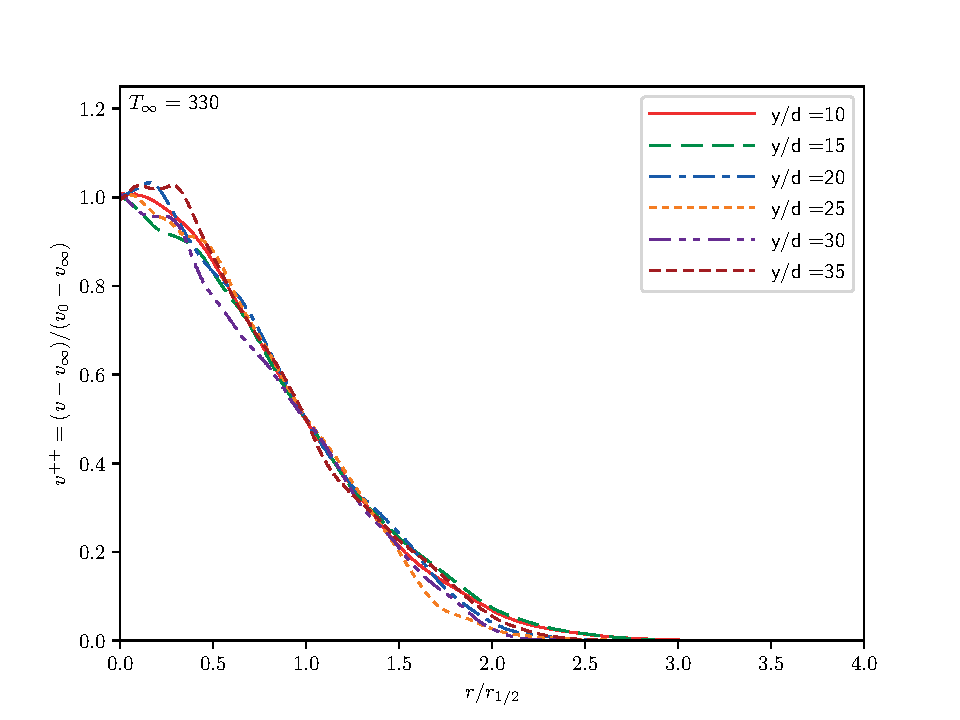
\includegraphics[scale=.45]{figures/Plots/radial/slices_5/same_ambient/r_vs_v.pdf}
	\caption{Far-Field} \label{330_r_vs_v_2}
\end{subfigure}
\caption{Normal slices of scaled axial velocity, averaged in both time and the radial direction. Plotted against radial direction scaled by $r_{1/2}$. Both near- and far-field regions demonstrate the self-similarity within the round turbulent jet.}
\label{330_r_v_features}
\end{center}
\end{figure}

Another common feature of round turbulent jets is the development of a linear relationship between the jet centerline value and the distance downstream. This comparison is depicted in Figure \ref{330_centerline_scaling}. Here, the centerline value of the axial velocity $v_0$ is inversely linearly proportional to the distance downstream. The dip at $\nicefrac{y}{d}=30$ may be attributed to again lack of convergence due to low sample size in time averaging. 

\begin{figure}[H]
\begin{center}
	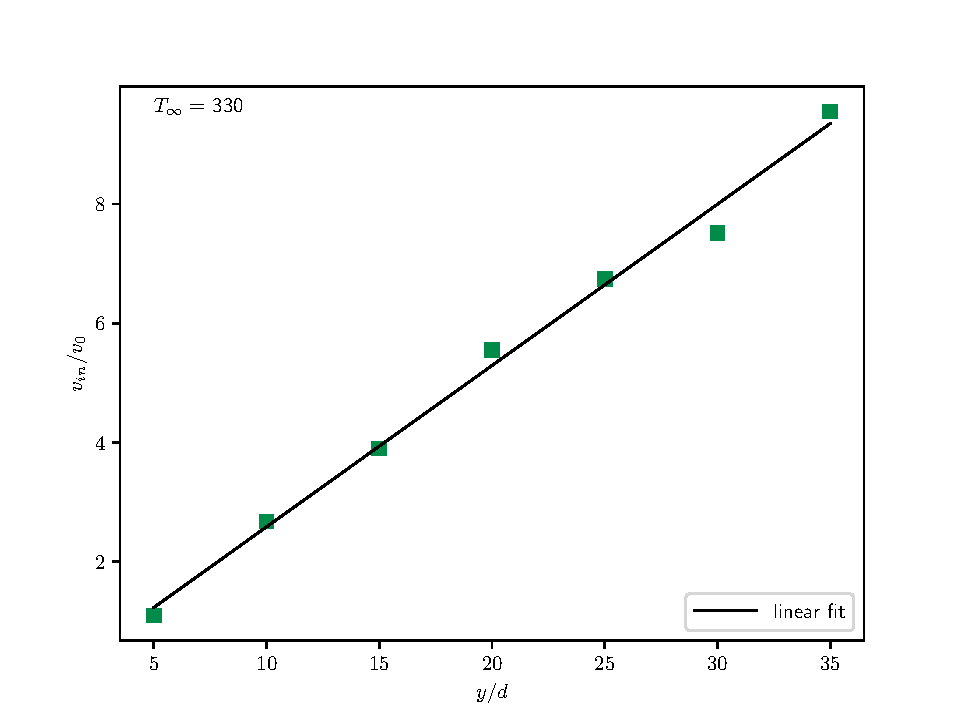
\includegraphics[scale=.7]{figures/Plots/radial/slices_5/same_ambient/uin_u0_vs_x_d.pdf}
	\caption{Axial inlet velocity scaled by centerline values along the axial direction. When distance downstream is scaled by jet diameter, linear decay of the centerline axial velocity is observed.} \label{330_centerline_scaling}
\end{center}
\end{figure}

\subsection{Turbulence Dynamics}
Figure \ref{330_reynolds_features} shows the time and radially averaged Reynolds stresses at two points downstream from the inlet. 

\begin{figure}[H]
\begin{center}
\begin{subfigure}{0.45\textwidth}
	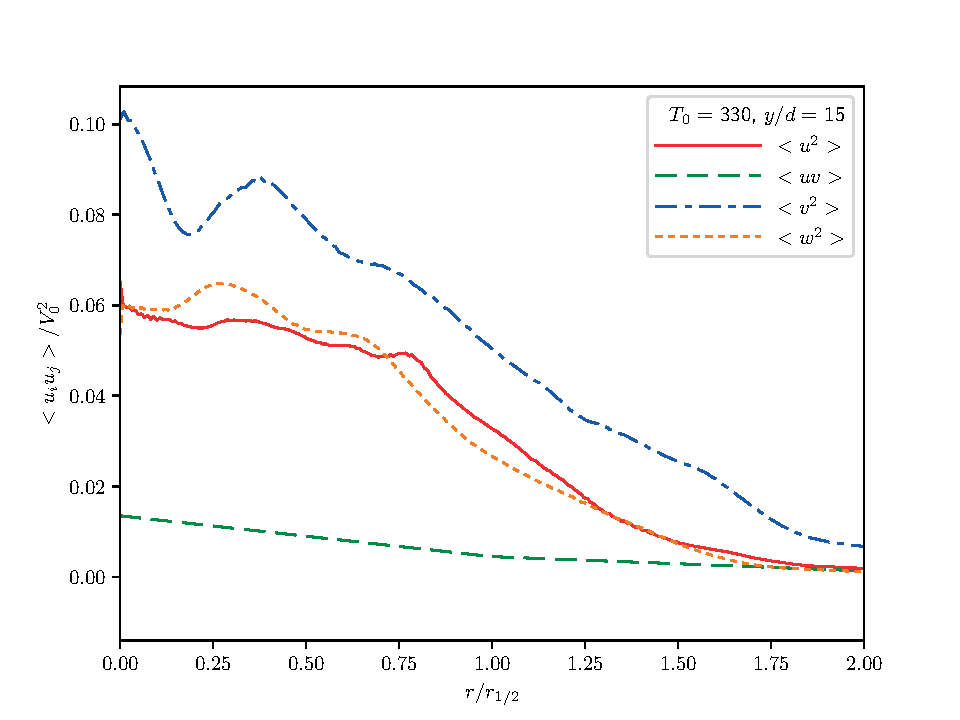
\includegraphics[scale=.45]{figures/Plots/radial/slices_5/same_ambient/Rey_Stress_0_15.pdf}
	\caption{Reynolds stresses at $y/d=15$} \label{330_rey_15}
\end{subfigure}
\begin{subfigure}{0.45\textwidth}
	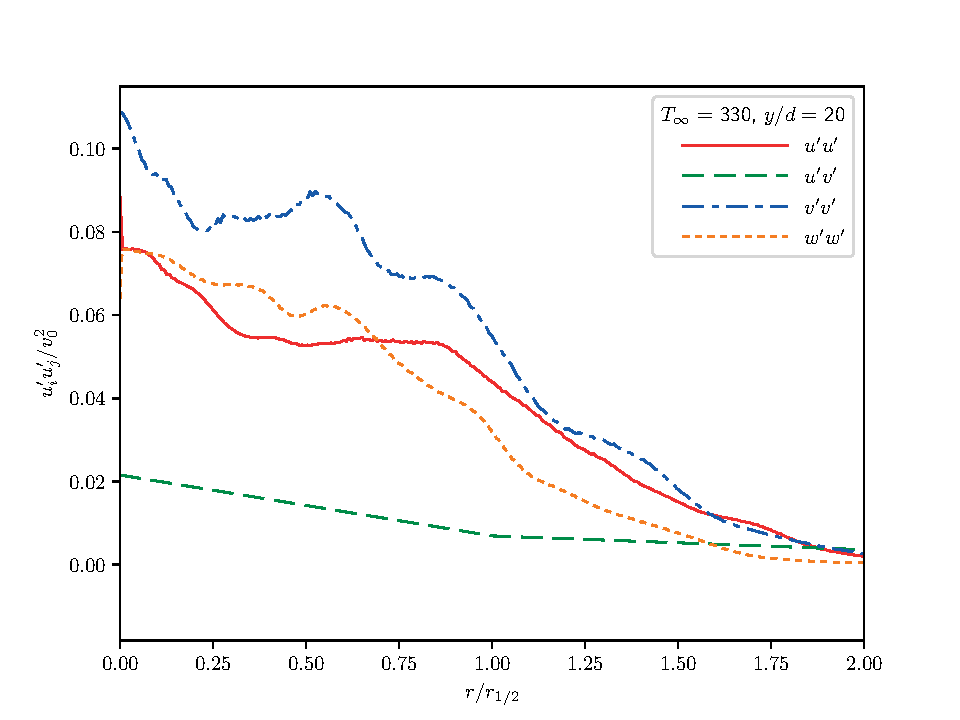
\includegraphics[scale=.45]{figures/Plots/radial/slices_5/same_ambient/Rey_Stress_0_2.pdf}
	\caption{Reynolds stresses at $y/d=20$} \label{330_rey_20}
\end{subfigure}
\caption{Time and radially averaged Reynolds stresses for the isothermal jet at two locations downstream. Both slices follow similar Reynolds stress relations as seen in incompressible round jet \cite{Pope}.}
\label{330_reynolds_features}
\end{center}
\end{figure}

\begin{figure}[H]
\begin{center}
	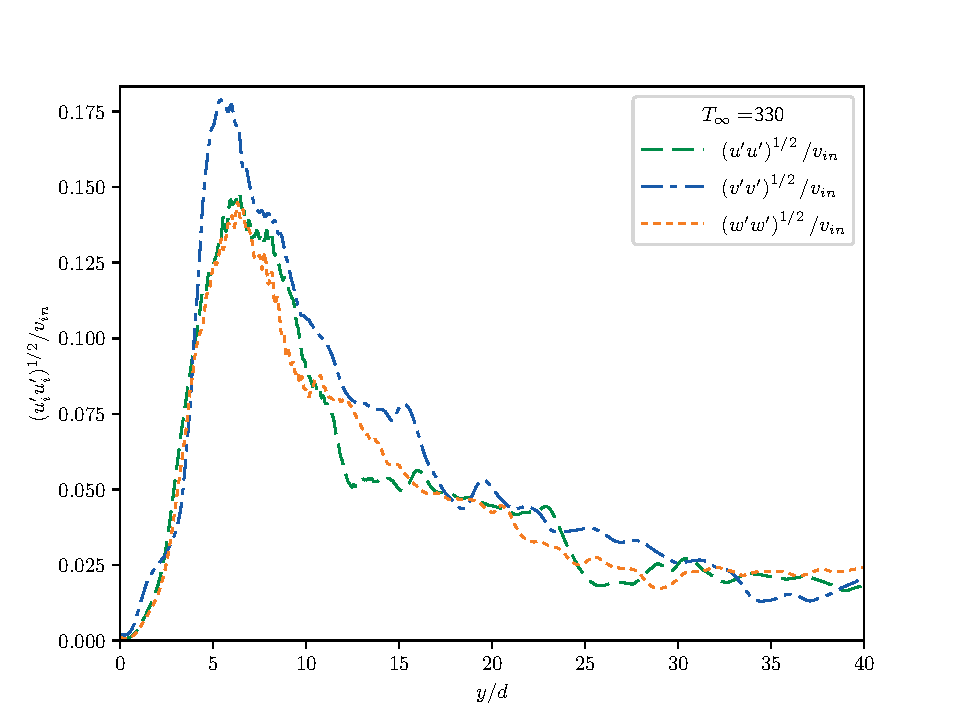
\includegraphics[scale=.7]{figures/Plots/centerline/330_TKEuvw_centerline.pdf}
	\caption{Average turbulent kinetic energy components along centerline.} \label{330_TKE_features}
\end{center}
\end{figure}

\section{Non-Isothermal Jets}
\subsection{Flow Field Features}

\subsection{Mean Flow Properties}
\subsection{Turbulence Dynamics}
\section{Discussion}



